%%%% début de la page
\teteSndCorp


%%%% titre
\nomPrenomClasse
\vspace{-12pt}
\numeroActivite{3}
\titreTP{Séparer et identifier des espèces chimiques}


%%%% objectifs
\begin{objectifs}
  \item Réaliser une Chromatographie sur Couche Mince.
  \item Renforcer ses connaissances sur le matériel de chimie.
\end{objectifs}


%%%% evaluation
\begin{tableauCompetences}
  \centering APP --
  Rechercher l'information.
  & & & &
  \\ \hline
  %
  \centering ANA/RAI --
  Justifier un protocole.
  & & & &
  \\ \hline
  %
  \centering REA --
  Mettre en \oe{}uvre un protocole.
  & & & &
  \\ \hline
  %
  \centering VAL --
  Comparer avec des valeurs de références.
  & & & &
\end{tableauCompetences}



%%%% contexte
\begin{encart}
  \emphase{Contexte :}
  
  En Europe, les colorants alimentaires sont désignés par un préfixe E suivi d'un numéro.
  Ces colorants se retrouvent dans de nombreux produits.
  
  On cherche à déterminer les colorants présent dans du sirop à l'aide d'une \textbf{Chromatographie sur Couche Mince (CCM).}
\end{encart}


%%%% document
\begin{doc}{Chromatographie sur Couche Mince (CCM)}
  \vspace*{-32pt}
  \begin{wrapfigure}{r}{0.5\linewidth}
    \centering
    \image{1}{images/CCM/CCM_exp.png}
    \footnotesize{Schéma expérimental d'une CCM.}
  \end{wrapfigure}

  La \important{chromatographie sur couche mince (CCM)} permet de séparer et d'identifier des espèces chimiques présentes dans un mélange.

  Le principe est le suivant : on dépose les espèces à identifier sur une couche mince (plaque), appelée \important{phase stationnaire}, dont on fait tremper une partie dans un \important{éluant}.
  
  Par capillarité, cet éluant va monter le long de la plaque, on parle de \important{phase mobile.}
  Les espèces déposées sur la plaque vont être entraînées par cette phase mobile.
  
  En fonction de leur affinités, les espèces chimiques monteront plus ou moins haut sur la plaque, ce qui permettra de les identifier.
  La fiche ainsi formée est appelée \important{chromatogramme}.
\end{doc}

%%%%
\begin{doc}{Lecture d'un chromatogramme}
  \vspace*{-24pt}
  \begin{wrapfigure}{r}{0.4\linewidth}
    \vspace*{-30pt}
    \centering
    \image{0.9}{images/CCM/chromatogramme_TP.png}
  \end{wrapfigure}
  
  \textbullet\hspace{2pt} \textbf{Lecture verticale :} si le dépôt d'un échantillon se sépare en plusieurs tâches, il s'agit d'un mélange.
  
  \textbullet\hspace{2pt} \textbf{Lecture horizontale :} sur une même plaque, une même espèce chimique migre toujours à la même hauteur.
 
  \vspace{20pt}
  \phantom{4}
\end{doc}

%%%%
\begin{doc}{Colorants alimentaires}
  \vspace*{-18pt}
  \begin{itemize}[label=\textbullet]
    \item \textbf{E102 : jaune de tartrazine.} Son usage doit s'accompagner en France de la mention \og peut avoir des effets indésirables sur l'activité et l'attention chez les enfants \fg.
    \item \textbf{E133 : bleu brillant.} Un enfant de 40 kg peut ingérer jusqu'à $240\unit{mg}$ de bleu brillant en une journée. Au-delà le conseil européen indique que ce produit peut être toxique.
  \end{itemize}
\end{doc}

%%%%
\begin{doc}{Réalisation d'une CCM}
  \vspace*{1pt}
  
  \separationTroisBlocs{
    \begin{center}
      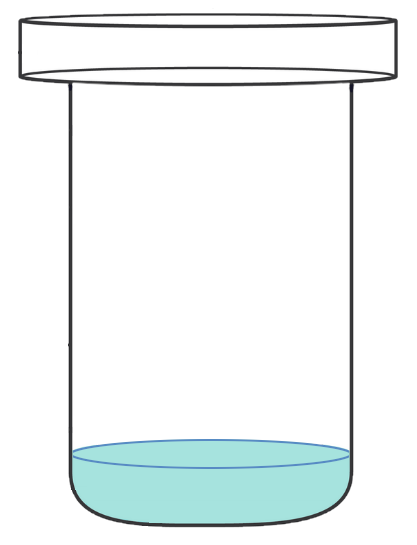
\includegraphics[height=0.15\textheight]{images/CCM/CCM_etapes_cuve.png}
    \end{center}
    
    \vspace*{-12pt}
    Remplir jusqu'à environ 0,5 cm de hauteur d'éluant la cuve à CCM.
  }{
    \begin{center}
      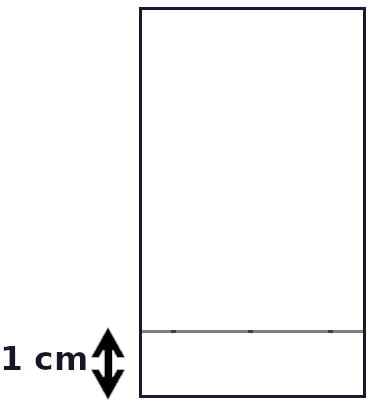
\includegraphics[height=0.15\textheight]{images/CCM/CCM_etapes_trait.png}
    \end{center}
    
    \vspace*{-12pt}
    À environ 1 cm du bord inférieur, tracer au crayon à papier un trait fin.
    Vérifier que le trait est au-dessus du niveau de l'éluant.
  }{
    \begin{center}
      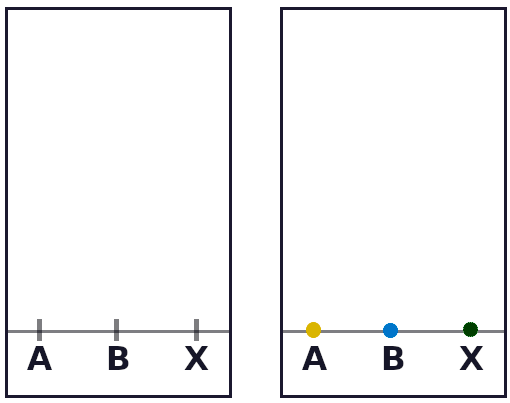
\includegraphics[height=0.15\textheight]{images/CCM/CCM_etapes_depot.png}
    \end{center}
    
    \vspace*{-12pt}
    Marquer les emplacements des échantillons à déposer.
    Prélever chaque échantillon avec un cure dent et les déposer sur l'emplacement prévu.
  }
  
  \bigskip
  
  \separationDeuxBlocs{
    \begin{center}
      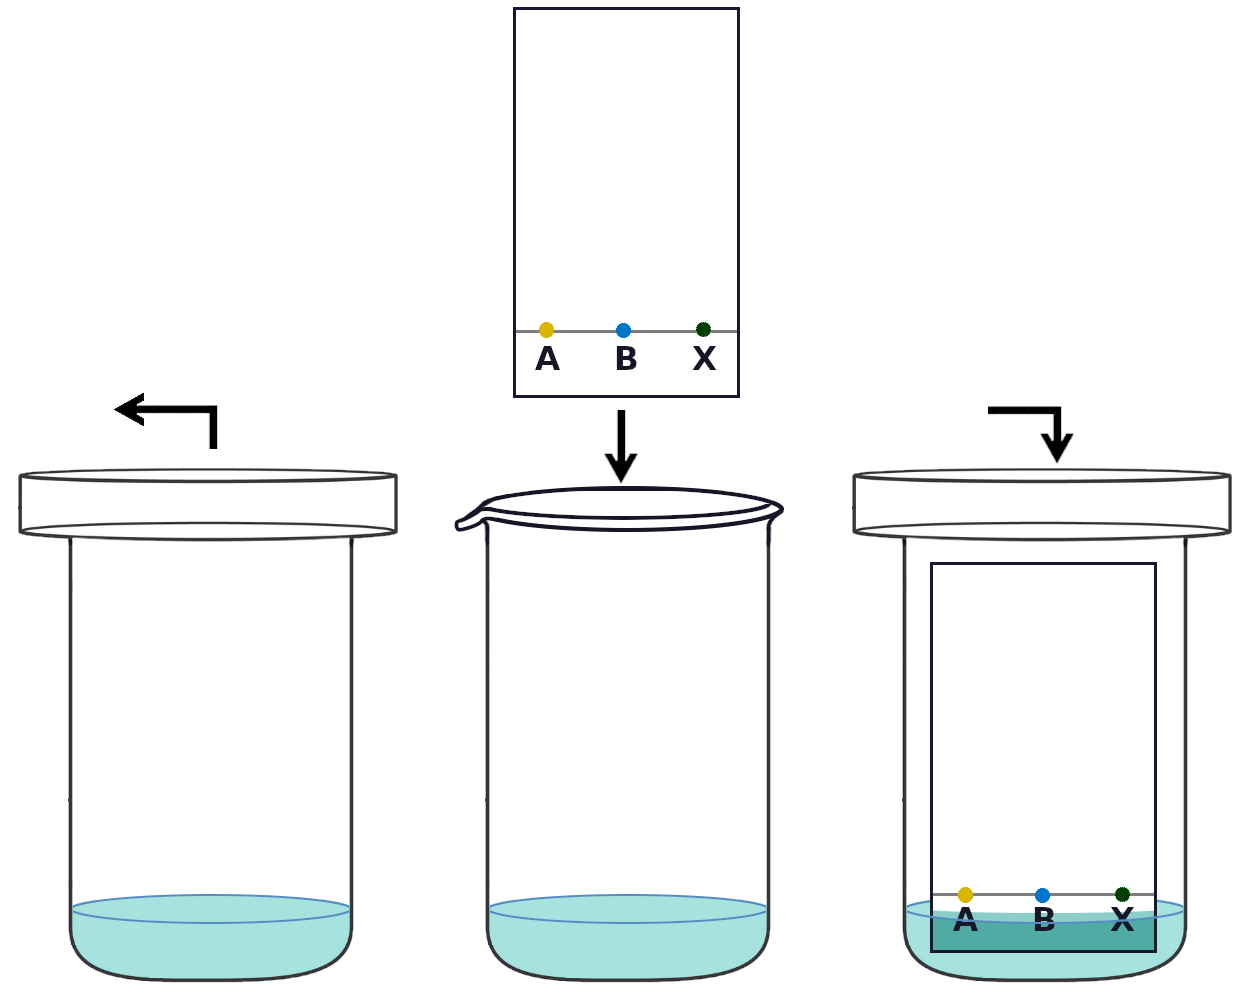
\includegraphics[height=0.25\textheight]{images/CCM/CCM_etapes_ajout.png}
    \end{center}
    
    \vspace*{-12pt}
    Introduire délicatement la plaque dans la cuve en la tenant par les côtés.
    Refermer la cuve.
    \textbf{Ne jamais déplacer la cuve} et attendre que l'éluant monte.
  }{
    \begin{center}
      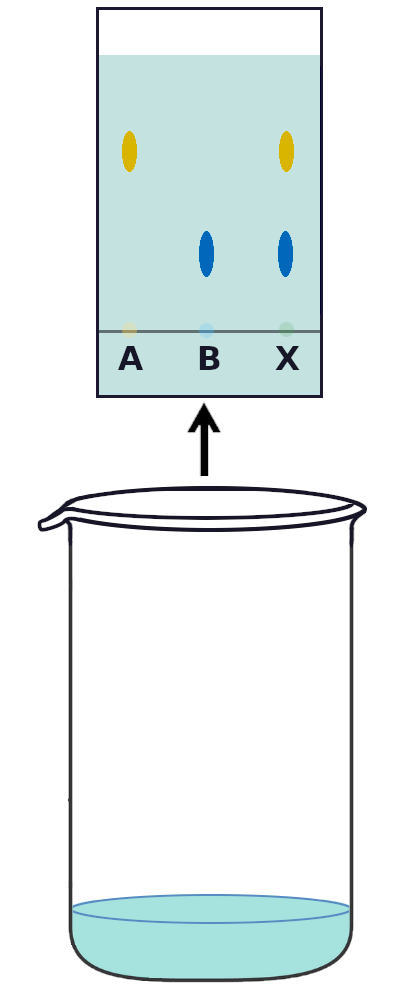
\includegraphics[height=0.25\textheight]{images/CCM/CCM_etapes_retrait.png}
    \end{center}
    
    \vspace*{-12pt}
    Quand le front de l'éluant s'approche du bord supérieur, sortir la plaque.
    Tracer immédiatement une ligne indiquant la hauteur où l'éluant est monté.
  }
\end{doc}


%%%% questions
\question{
  Placer quelques gouttes de sirop vert dans un bécher de $50\unit{mL}$. Ajouter environ $10\unit{mL}$ d'eau distillée et agiter.\competence{REA}
}{0}

\question{
  Réaliser le protocole du document 3, avec un dépôt de colorant jaune, un dépôt de colorant bleu et  et un dépôt de la solution préparée à la question 1.\competence{REA}
}{0}

\question{
  Coller ici le chromatogramme \textbf{sec} et entourer les différentes tâches au crayon à papier.\competence{REA}
}{0}
\vspace*{240pt}

\newpage
\question{
  Pourquoi doit-on placer la ligne de dépôt au dessus du niveau de l'éluant ?\competence{ANA/RAI}
}{2}

\question{
  Pourquoi ne doit-on pas déplacer la cuve pendant la montée de l'éluant ?\competence{ANA/RAI}
}{2}

\question{
  En analysant le chromatogramme à l'aide du document 2, indiquer si les échantillons sont des corps purs ou des mélanges.\competence{APP}
}{3}

\question{
  En utilisant le chromatogramme, que contient le colorant vert du sirop ? Justifier avec des arguments simples.\competence{APP, VAL}
}{2}


% \newpage
% \question{Relier chaque verrerie à son nom.}{0}

% %%
% \newcommand{\centeredBullet}{\centering\textbullet}
% \vspace*{-12pt}
% \begin{center}
%   \image{1}{images/instruments_chimie/instruments_1.png}
  
%   \begin{tabular}{
%     m{0.23\textwidth} m{0.23\textwidth} m{0.23\textwidth} m{0.23\textwidth} m{12pt}
%   }
%     \centeredBullet & \centeredBullet & \centeredBullet & \centeredBullet & \phantom{b}
%     \\[48pt]
%     \centeredBullet & \centeredBullet & \centeredBullet & \centeredBullet & \phantom{b}
%     \\
%     \centering sabot de pesée  &  \centering tube à essai  &  \centering coupelle de pesée  & \centering verre à pied &
%   \end{tabular}
% \end{center}

% %%
% \vspace{12pt}
% \begin{center}
%   \image{1}{images/instruments_chimie/instruments_2.png}
  
%   \begin{tabular}{
%     m{0.21\textwidth} m{0.23\textwidth} m{0.25\textwidth} m{0.28\textwidth} m{12pt}
%   }
%     \centeredBullet & \centering\textbullet & \centeredBullet & \centeredBullet & \phantom{b}
%     \\[48pt]
%     \centeredBullet & \centeredBullet & \centeredBullet & \centeredBullet & \phantom{b}
%     \\
%     \centering éprouvette graduée  &  \centering bécher &  \centering fiole jaugée  & \centering erlenmeyer &
%   \end{tabular}
% \end{center}
